\documentclass[12pt]{article}
\usepackage[caption=false]{subfig}
\usepackage[utf8]{inputenc}
\usepackage{amsmath}
\usepackage{bbding}
\usepackage{cases}
\usepackage{amsfonts}
\usepackage{mathrsfs}
\usepackage{amssymb}
\usepackage{graphicx}
% \usepackage{enumerate}
% \usepackage{datetime}
\usepackage{paralist}
\usepackage{multirow}
% \usepackage[ruled,linesnumbered]{algorithm2e}
%\usepackage{subfigure}
%\usepackage{indentfirst}
\usepackage{color}
\usepackage [top=0.8in, bottom=1in, left=2cm, right=2cm]{geometry}
% \setlength{\parindent}{2em}
\usepackage{parskip}  % 加载宏包,实现段落间有空白、首行无缩进
% \usepackage{algorithmic}
\usepackage{algorithm}
\usepackage{algpseudocode}
\usepackage{caption}
\usepackage{subcaption}  % 加载 subcaption 宏包
\usepackage{float}% http://ctan.org/pkg/float
\usepackage{nicematrix}
\usepackage{tikz} % For drawing step lines
%\usepackage{tikz}
\usetikzlibrary{matrix,decorations.pathreplacing}
% \usepackage{todonotes}
\newtheorem{theorem}{Theorem}[section]
\newtheorem{definition}[theorem]{Definition}
%\newtheorem{algorithm}[theorem]{Algorithm}
\newtheorem{lemma}[theorem]{Lemma}
\newtheorem{corollary}[theorem]{Corollary}
\newtheorem{proposition}[theorem]{Proposition}
\newtheorem{example}[theorem]{Example}
\newtheorem{remark}[theorem]{Remark}
% \newenvironment{proof}{\noindent {\bf Proof.\ }}{$\blacksquare$\vspace{2ex}}
\newenvironment{proof}{\noindent {\bf Proof.\ }}{\vspace{2ex}}

\numberwithin{equation}{section} % 将方程编号关联到章节,若用 chapter 就改 \section 为 \chapter
\usepackage[noadjust]{cite}

\newcommand{\red}{\color{red}}


\usepackage{lipsum}
\usepackage{arydshln}
\newcommand\blfootnote[1]{%
  \begingroup
  \renewcommand\thefootnote{}\footnote{#1}%
  \addtocounter{footnote}{-1}%
  \endgroup
}

\begin{document}
\begin{center}
    {\LARGE \textbf{An Algorithm for QR Decomposition of  Split Quaternion Matrices} 
    \blfootnote{This
research is supported by Macao Science and Technology Development Fund (No. 0013/2021/ITP), the grants from the National Natural Science Foundation of China (12371023, 12271338), and the Natural Sciences and Engineering Research Council of Canada (NSERC) (RGPIN 2020-06746), The joint research and Development fund of Wuyi University, Hong Kong and Macao (2019WGALH20), Macau University of Science and Technology
Faculty Research Grants (FRG-22-073-FIE) \par
* Corresponding author
E-mail: xiliu@must.edu.mo}}
\bigskip
$${\large \textbf{Qianqian Liu}^{1},  \textbf{Xin Liu}^{1, \ast}, \textbf{Jianhai Lin}^{1},\textbf{Yang Zhang}^{2}}$$
\newline $^{\text{1}}$Faculty of Innovation Engineering, Macau University of Science and Technology,
\newline Avenida Wai Long, TaiPa, Macau, 999078, P. R. China.
\newline $^{\text{2}}$ Department of Mathematics, University of Manitoba,
\newline Winnipeg, MB, R3T 2N2, Canada.\\
\end{center}
\begin{abstract}
Split quaternions contain zero divisors, thus it is not a Euclidean distance space. Therefore, the traditional QR decomposition based on Givens rotations and Householder reflection transformations is difficult to implement. To overcome this difficulty and to address the non-commutativity of split quaternion multiplication, we will utilize the real representation $A^\sigma$ of the split quaternion matrix $A$.  By leveraging the proposed decomposition $A^\sigma = \hat{Q}R_4$  ($\hat{Q}$ is an orthogonal matrix, and $R_4 = \begin{bmatrix}
    R_{11} & R_{12} \\
    R_{21} & R_{22}
\end{bmatrix}$, with $R_{11}, R_{12}, R_{21}, R_{22}$ being upper triangular), the QR decomposition of the split quaternion matrix was successfully constructed using its real representations. To verify its effectiveness, the proposed algorithm was used for QR decomposition and solving a matrix equation, and the experimental results demonstrate its high efficiency in CPU Time and accuracy.
\iffalse
    Split quaternion matrices play a vital role in signal processing and quantum computing, yet the QR decomposition of split quaternion matrices has not been fully resolved. This paper establishes and rigorously proves the QR decomposition theorem for split quaternion matrices through their real representation matrices. We design a corresponding algorithmic framework and elucidate the construction of the upper triangular matrix $R$ in the decomposition. Experimental results show that, compared to traditional algorithms, the proposed algorithm significantly reduces the computation time when handling QR decomposition of split quaternion matrices, effectively improving computational efficiency. Moreover, it demonstrates excellent performance in error control, with higher accuracy of decomposition results, greatly reducing result deviations caused by cumulative computational errors.
\fi

    \noindent\textbf{Key words:}  Split quaternion matrix; QR decomposition; Permutation matrix; Upper triangular matrix.
\end{abstract}
\section{\textbf{Introduction}}
\iffalse
Quaternions, as a higher-dimensional generalization of complex numbers, have exhibited irreplaceable theoretical value in fields such as computer graphics (3D rigid body rotation), quantum mechanics (spin state description) and aerospace navigation (attitude control) since Hamilton proposed them in 1843. In particular, for tasks such as optimization of 3D space rotation transformations and multi-channel color image processing, quaternion matrix decomposition methods have become key mathematical tools in related fields due to their inherent structure-preserving properties and computational efficiency advantages.\fi


In 1849, James Cockle \cite{Cockle1849} introduced the concept of split quaternion algebra over the real numbber field $\mathbb{R}$,   which can be described by the following rules:
\[
\mathbb{H}_s = \{ a_1 + a_2 i + a_3 j + a_4 k \mid i^2 = -1, \quad j^2 = k^2 = 1, \quad ijk = 1, \quad \text{and} \quad a_1, a_2, a_3, a_4 \in \mathbb{R} \}.
\] 
\iffalse
$\mathbb{H}_s$, as a four-dimensional non-commutative associative algebra, it belongs to the category of Clifford algebras. However, the non-uniform sign characteristics of its imaginary units ($j^2 = k^2 = 1$) endow it with unique hyperbolic geometric properties, which makes split quaternion matrices show significant application potential in interdisciplinary fields such as quantum field theory (spacetime symmetry modeling), biomedical signal processing (multimodal data fusion) and coding theory (error-correcting code construction)\cite{TJiang2015}-\cite{Kula2016}. In recent years, systematic research on the algebraic properties of split quaternions has made remarkable progress. References \cite{Yasemin2012}-\cite{Yang2020} have deepened the theoretical system from the perspectives of invertibility conditions, spectral theory, and polynomial equation solving, providing new paradigms for mathematical modeling of related engineering problems.
\fi
$\mathbb{H}_s$ is a four dimensional commutative algebra over $\mathbb{R}$ and contains zero divisors.  The matrices over $\mathbb{H}_s$ have been found many applications in quantum mechanics, electromagnetism, signal processing, and coding theory (see, e.g., \cite{Hasebe2010}-\cite{Wang2023}). In the past  decades, many researches  have been done in studying the algebraic properties of split quaternions (see, e.g., \cite{Yasemin2012}-\cite{Gang2024}, \cite{wang},  \cite{mma}, \cite{yuan}). For example, \cite{Zhang2015} solved the least squares problem of the split quaternion matrix equation $AX=B$; \cite{Jiang2018}-\cite{TJiang2018} respectively solved the eigenvalue problems and the solutions to the Schrödinger equation; \cite{wang}   solved the classical system of matrix equations; \cite{Wang2021} proposed a fast algorithm based on LDU decomposition; \iffalse 
\cite{Gang2024} proposed the singular value decomposition for the split quaternion matrix, presenting the SVD theorem and the corresponding algorithms for such matrices. However, existing research has not completely solved the theoretical construction and algorithm implementation of QR decomposition for split quaternion matrices. 
\fi 
\cite{Gang2024}  proposed the SVD decomposition theory and an efficient algorithm for decomposing quaternion matrices. \iffalse This work has been successfully applied to 3D wave denoising, yielding favorable outcomes.\fi However, the existing research has yet to fully address the theoretical development and algorithmic implementation of QR decomposition for split quaternion matrices.

To address the above problem, we constructively prove the existence of QR decomposition for split quaternion matrices, and we propose a novel and efficient algorithm for computing this QR decomposition.  To validate the efficiency  of our algorithm, we provide the experimental results in terms of speed and accuracy.


\iffalse Additionally, the algorithm is applied to solve split quaternion matrix equations. The experimental results indicate that the proposed algorithm is an efficient method and can effectively solve the problem of finding solutions to split quaternion matrix equations.
\fi
\iffalse
this paper designs a comparative experiment to evaluate the performance of the proposed method and Sangwine's QR algorithm\cite{Gang2024}. The experimental results show that the new algorithm has significant advantages in both the calculation time and the numerical residual, which confirms its value in engineering application.
 

The core contributions of this study are reflected in three aspects: 

1. Algebraic structure preservation mechanism: The split quaternion matrix is transformed into a real matrix representation through an isomorphic mapping to completely retain its algebraic constraints; a P-permutation operator is introduced to preprocess the real matrix, effectively eliminating the subspace orthogonality distortion caused by traditional real embedding.  

2. Optimization of computational efficiency: After performing the standard QR decomposition in the real matrix domain, the upper triangular matrix is reconstructed by inverse permutation and algebraic constraints, significantly reducing the computational complexity (theoretical analysis shows that the calculation amount is reduced to 72\% of the traditional method).

3. Theoretical framework extensibility: The proposed method provides a unified numerical analysis framework for derivative problems such as eigenvalue calculation and minimum-norm solution of split quaternion matrices.  
\fi


\section{\textbf{Preliminaries}}
For any split quaternion matrix \({A}=A_{1}+A_{2}i + A_{3}j + A_{4}k \in\mathbb{H}_{s}^{m\times n}\), where \(A_{i}\in\mathbb{R}^{m\times n}, i\in\{1,2,3,4\}\), its transpose, conjugate, conjugate transpose, i-conjugate, and i-conjugate transpose are  denoted by 
 \({A}^T = A_1^T + A_2^Ti + A_3^Tj + A_4^Tk,\bar{{A}} = A_1 - A_2i - A_3j - A_4k, {A}^* = A_1^T - A_2^Ti - A_3^Tj - A_4^Tk,\) and \(\tilde{{A}} = A_1 - A_2i + A_3j + A_4k,{A}^H = A_1^T - A_2^Ti + A_3^Tj + A_4^Tk\), respectively.

The real representation matrix of a split quaternion matrix is presented as \cite{TJiang2015}:
\begin{equation}
{A}^\sigma = \begin{bmatrix} A_1 + A_3 & -A_2 + A_4 \\ A_2 + A_4 & A_1 - A_3 \end{bmatrix} \in \mathbb{R}^{2m \times 2n},\label{eq:2.1}
\end{equation}
which has the properties
\begin{equation}
    ({A} + {B})^\sigma = {A}^\sigma + {B}^\sigma, \quad ({A}{C})^\sigma = {A}^\sigma {C}^\sigma, \quad (a {A})^\sigma = a {A}^\sigma, \ (t{A}^H)^\sigma = ({A}^\sigma)^H\label{eq:2.1.1},
\end{equation}
where ${A}, {B} \in \mathbb{H}_s^{m \times n}$, ${C} \in \mathbb{H}_s^{n \times p}$, $a \in \mathbb{R}$.

\iffalse 
By direct verification, it is established that the conjugate transpose of the real representation matrix \(A^\sigma\) does not generally equal the conjugate transpose of \(A\), i.e.,
In general, \((A^*)^\sigma \neq (A^\sigma)^*\). However, for the i-conjugate transpose \(A^H\), the equality holds, \((A^H)^\sigma = (A^\sigma)^H\). 
\fi

Furthermore,  \({A}\) is called unitary if \({A}{A}^H = {A}^H {A} = I\). We can verify that \(A\) is unitary if and only if  \({A}^\sigma\) is  orthogonal (\cite{TJiang2018}).
 The Frobenius norm of \({A}\) is defined as: $ \| {A} \|_F \equiv \frac{1}{\sqrt{2}} \| {A}^\sigma \|_F = \sqrt{\| A_1 \|_F^2 + \| A_2 \|_F^2 + \| A_3 \|_F^2 + \| A_4 \|_F^2}.$ When ${U}, {V}$ are unitary, ${U}^\sigma$ and ${V}^\sigma$ are orthogonal, which will not change the Frobenius norm  of $A^\sigma$. Hence
$\|{U}{A}{V}\|_F = \frac{1}{\sqrt{2}} \|({U}{A}{V})^\sigma\|_F 
= \frac{1}{\sqrt{2}} \|{U}^\sigma {A}^\sigma {V}^\sigma\|_F
=\frac{1}{\sqrt{2}} \|{A}^\sigma\|_F
= \|{A}\|_F.$

For any real matrix $B = \begin{bmatrix} B_{11} & B_{12} \\ B_{21} & B_{22} \end{bmatrix} \in \mathbb{R}^{2m \times 2n}$, $B_{ts} \in \mathbb{R}^{m \times n}$, $t, s = 1, 2$, one can construct a corresponding split quaternion matrix \(A\) as follows \cite{TJiang2015}:
\begin{equation}
{A} = \frac{B_{11} + B_{22}}{2} + \frac{B_{21} - B_{12}}{2}i + \frac{B_{11} - B_{22}}{2}j + \frac{B_{21} + B_{12}}{2}k.\label{eq:2.2}
\end{equation}
From equation \eqref{eq:2.1}, we have ${A}^\sigma = B$. 

{\color{red} $\sigma$ provides an one-to-one corresponding between $\mathbb{H}^{m\times n}$ and $\mathbb{R}^{2m \times 2n}$ ??? well-known? cite from which paper? }

%\begin{corollary}
\iffalse
A permutation matrix $P$ is invertible and satisfies $P^{-1} = P^T$, which means that it is also an orthogonal matrix.\fi
%\end{corollary}
\iffalse
\begin{lemma}\label{unitary}
    An $m \times n$ split quaternion matrix $A$ is unitary if and only if
    \[AA^H =A^H A = I\]
\end{lemma}

\begin{lemma}\label{unitary matrix}
    If a matrix $A\in \mathbb{R}^{m\times n}$ is a unitary matrix, then $PAP^T$ is also a unitary matrix, where $P$ is a permutation matrix.
\end{lemma}
\fi
\section{\textbf{QR Decomposition of Split Quaternion matrix}}
In this section, we prove the QR decomposition for split quaternion matrices through construction, and based on this, we propose an efficient algorithm.

We construct the QR decomposition of $A \in \mathbb{H}^{m \times n}$ as follows:

\textbf{Step 1:} Perform the decomposition of $A^\sigma \in \mathbb{R}^{2m \times 2n}$ as \begin{equation}\label{splitqr}A^\sigma = \hat{Q} R_4,\end{equation} where $\hat{Q}$ is an orthogonal matrix, and $R_4$ is a block matrix given by:
\begin{equation}\label{r4}
R_4 = \begin{bmatrix}
    R_{11} & R_{12} \\
    R_{21} & R_{22}
\end{bmatrix} \in \mathbb{R}^{2m \times 2n},
\end{equation}
and $R_{11}, R_{12},R_{21},R_{22}$ are all upper triangular matrices with size of  $m \times n$.

To achieve the special decomposition \eqref{splitqr},  we will first figure out how to transform an upper triangular matrix $R$ into $R_4$ through permutation transformations, as depicted in Figure 1.
\begin{figure}[htbp]
    % \begin{minipage}[htbp]{0.45\textwidth}
        \centering
        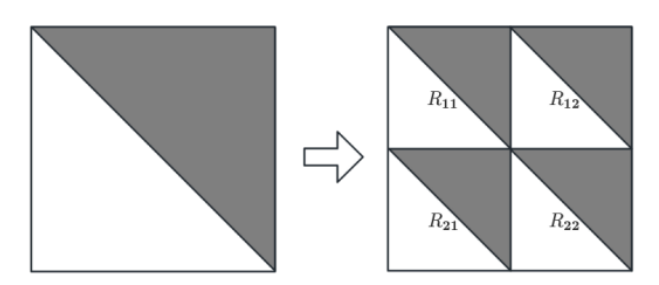
\includegraphics[width=0.45\textwidth]{Upper triangular.png} % Replace with actual file name
         % \caption{Transformation of a $2n \times 2n$ upper triangular matrix.}
         \label{fig:Upper triangular}
    % \end{minipage}
\end{figure}
 It is the key to realize the special decomposition \eqref{splitqr}. To better understand the procedure, we will choose the matrix 
\[R= \begin{bmatrix}
\begin{array}{cc:cc:cc}
 r_{11} & r_{12} & r_{13} & r_{14} & r_{15} & r_{16}\\
 0 & r_{22} & r_{23} & r_{24} & r_{25} & r_{26}\\
 \cdashline{1-6}
 0      & 0      & r_{33} & r_{34} & r_{35} & r_{36}\\
 0      & 0      & 0 & r_{44} & r_{45} & r_{46}\\
 \cdashline{1-6}
 0      & 0      & 0      & 0      & r_{55} & r_{56}\\
 0      & 0      & 0      & 0      & 0 & r_{66}\\
\end{array}
\end{bmatrix}
\]
to demonstrate. 

By performing the following swaps in matrix $R_2$: Replace the odd rows (1, 3, 5) sequentially with the first three rows. Replace the even rows (2, 4, 6) sequentially with the last three rows. Replace the odd columns (1, 3, 5) sequentially with the first three columns. Replace the even columns (2, 4, 6) sequentially with the last three columns. We can obtain the following  resulting matrix:

\[R_4 = \begin{bmatrix}
\begin{array}{ccc:ccc}
 r_{11} & r_{13} & r_{15} & r_{12} & r_{14} & r_{16}\\
 0      & r_{33} & r_{35} & 0      & r_{34} & r_{36}\\
 0      & 0      & r_{55} & 0      & 0      & r_{56}\\
 \cdashline{1-6}
0 & r_{23} & r_{25} & r_{22} & r_{24} & r_{26}\\
 0      & 0 & r_{45} & 0      & r_{44} & r_{46}\\
 0      & 0      & 0 & 0      & 0      & r_{66}\\
\end{array}
\end{bmatrix}=\begin{bmatrix}
    R_{11} & R_{12}\\R_{21} & R_{22}
\end{bmatrix}.
\]
To obtain the matrix $P$ for $R \in \mathbb{R}^{2m \times 2n}$, we established Algorithm \eqref{alg:Permutation}. When the input is $A=I$ and $flag=0$, we can obtain the matrix $P$, see equation  \ref{p}. It can be expressed as:
\begin{equation}
    P_{m} R P_{n}^T = \begin{bmatrix} R_{11} & R_{12}\\R_{21}& R_{22}\end{bmatrix},\label{eq:Rn}
\end{equation}
where
\begin{equation}\label{p}
    P_k = \begin{bmatrix} 
            1 & 0 & 0 & 0 & \cdots & 0 & 0\\ 
            0 & 0 & 1 & 0 & \cdots & 0 & 0\\ 
            \vdots & \vdots & \vdots & \vdots &  & \vdots & \vdots\\ 
            0 & 0 & 0 & 0 & \cdots & 1 & 0 \\
            0 & 1 & 0 & 0 & \cdots & 0 & 0\\ 
            0 & 0 & 0 & 1 & \cdots & 0 & 0\\ 
            \vdots & \vdots & \vdots & \vdots &  & \vdots & \vdots\\ 
            0 & 0 & 0 & 0 &\cdots & 0 & 1 
        \end{bmatrix}_{2k \times 2k}
\end{equation}
is a permutation matrix.
% {\color{red}When the upper triangular matrix $R$ is not a square matrix, equation \eqref{eq:Rn} still holds.} 

After completing the above steps, we can now proceed to implement the decomposition \eqref{splitqr}.
First, perform the QR decomposition to the real matrix $P_m^TA^\sigma P_{n}$:
\[P_m^TA^\sigma P_n = QR.\]
According to \eqref{eq:Rn}, we have
\[P_m^TA^\sigma P_n = QR = Q(P_m^TR_4P_n).\]
Multiplying both sides of the equation by $P_m$ on the left and $P_n^T$ on the right yields
\[A^\sigma=P_mQP_m^T R_4.\]
Since $P_m$ is a permutation matrix, it is also an orthogonal matrix. Therefore, the product of matrices, $P_mQP_m^T$, is also an orthogonal matrix, then we get our required special decomposition $A^\sigma=\hat{Q}R_4,$ where $\hat{Q}=P_mQP_m^T$ is orthogonal, and $R_4$ is in the form of \eqref{r4}.


\textbf{Step 2:} Using equation \eqref{eq:2.2}, construct the matrix $R$ such that $R^\sigma=R_4:$
$$
R = \frac{R_{11} + R_{22}}{2} + \frac{R_{21} - R_{12}}{2}i + \frac{R_{11} - R_{22}}{2}j + \frac{R_{21} + R_{12}}{2}k.
$$
Since $R_{11}, R_{12}, R_{21}, R_{22}$ are upper triangular, this ensures the constructed split quaternion matrix $R$ is also upper triangular.


Additionally, construct the matrix $Q$ such that $Q^\sigma=\hat{Q}:$
$$
Q = \frac{Q_{11} + Q_{22}}{2} + \frac{Q_{21} - Q_{12}}{2}i + \frac{Q_{11} - Q_{22}}{2}j + \frac{Q_{21} + R_{12}}{2}k.
$$
Here,  $Q_{11}, 
 Q_{12}, Q_{21}, Q_{22}$ are the blocks of the orthogonal matrix $\hat{Q} = \begin{bmatrix} Q_{11} & Q_{12} \\ Q_{21} & Q_{22} \end{bmatrix} \in \mathbb{
 R}^{2m \times 2m}$.

Note that $(Q^H Q)^\sigma = {(Q^H)}^\sigma Q^\sigma = {(Q^\sigma)}^TQ^\sigma = \hat{Q}^T\hat{Q} = I_{2m}$, indicating that the split quaternion matrix $Q$ remains a unitary matrix.
Now, $A^\sigma=\hat{Q}R_4=Q^\sigma R^\sigma$ implies
$A = Q R$, as required.

From the process described above,  any split quaternion matrix can be decomposed into QR decomposition. Our results can be summarized as follows:
\begin{theorem}(QR Decomposition)
    Let $A \in \mathbb{H}_s^{m \times n}$. There exist a unitary matrix $Q \in \mathbb{H}_s^{m \times m}$ and an upper triangular matrix $R \in \mathbb{H}_s^{m \times n}$ such that
    \begin{equation}
        A = Q R.\label{eq:split QR}
    \end{equation}
\end{theorem}

% \iffalse
% {\color{red}SO, No need the proof? }
% \begin{proof}
%    For any matrix $A \in \mathbb{H}_s^{m \times n}$, to prove that $A = Q R$ holds, according to the real representation form of split quaternions, it suffices to prove that
% \begin{equation}
%     A^\sigma = Q^\sigma R^\sigma,\label{eq:3.1}
% \end{equation}
% where $Q^\sigma \in \mathbb{R}^{2m\times 2m}$ is an orthogonal matrix, $R^\sigma = \begin{bmatrix}
%     R_{11} & R_{12}\\
%     R_{21} & R_{22}
% \end{bmatrix} \in \mathbb{R}^{2m\times 2m}$, and $R_{ij}$ ($i, j = 1, 2$) are $m\times n$ upper triangular matrices. 

% $R^\sigma$ can be obtained by permuting rows and columns of the following ladder-shaped matrix, as shown in Example \ref{example upper triangular}. 
% \[R_2 = 
% \begin{tikzpicture}[baseline=(current bounding box.center)]
% \matrix [matrix of math nodes,left delimiter={[},right delimiter={]}] (m) {
% * & * & * & * & * & * & \cdots & * & * & * & * \\
% * & * & * & * & * & * & \cdots & * & * & * & * \\
% 0 & 0 & * & * & * & * & \cdots & * & * & * & * \\
% 0 & 0 & * & * & * & * & \cdots & * & * & * & * \\
% 0 & 0 & 0 & 0 & * & * & \cdots & * & * & * & * \\ 
% 0 & 0 & 0 & 0 & * & * & \cdots & * & * & * & * \\ 
% \vdots & \vdots & \vdots & \vdots & \vdots & \vdots & \vdots & \vdots & \vdots & \vdots & \vdots \\ 
% 0 & 0 & 0 & 0 & 0 & 0 & \cdots & * & * & * & * \\ 
% 0 & 0 & 0 & 0 & 0 & 0 & \cdots & * & * & * & * \\ 
% 0 & 0 & 0 & 0 & 0 & 0 & \cdots & 0 & 0 & * & * \\ 
% 0 & 0 & 0 & 0 & 0 & 0 & \cdots & 0 & 0 & * & * \\
% };
% % Draw step lines
% \draw[thick] (m-1-1.north west) -- (m-2-1.north west) -- (m-3-1.north west) -- (m-3-2.north east) -- (m-3-2.south east) -- 
%              (m-4-2.south east) -- (m-4-2.south east) -- (m-4-4.south east) --
%              (m-4-4.south east) -- (m-6-4.south east) -- (m-6-6.south east)
%              (m-8-8.north west) -- (m-9-8.south west) --
%              (m-9-7.south east) -- (m-9-9.south east) 
%              --
%              (m-11-9.south east) -- (m-11-11.south east);
% \end{tikzpicture}_{2n \times 2n}
% \]

% \begin{example}\label{example upper triangular}
% \[R_2 = \begin{bmatrix}
% \begin{array}{cc:cc:cc}
%  r_{11} & r_{12} & r_{13} & r_{14} & r_{15} & r_{16}\\
%  r_{21} & r_{22} & r_{23} & r_{24} & r_{25} & r_{26}\\
%  \cdashline{1-6}
%  0      & 0      & r_{33} & r_{34} & r_{35} & r_{36}\\
%  0      & 0      & r_{43} & r_{44} & r_{45} & r_{46}\\
%  \cdashline{1-6}
%  0      & 0      & 0      & 0      & r_{55} & r_{56}\\
%  0      & 0      & 0      & 0      & r_{65} & r_{66}\\
% \end{array}
% \end{bmatrix}
% \]

% \[R_2 = \begin{bmatrix}
% \begin{array}{ccc:ccc}
%  r_{11} & r_{13} & r_{15} & r_{12} & r_{14} & r_{16}\\
%  0      & r_{33} & r_{35} & 0      & r_{34} & r_{36}\\
%  0      & 0      & r_{55} & 0      & 0      & r_{56}\\
%  \cdashline{1-6}
%  r_{21} & r_{23} & r_{25} & r_{22} & r_{24} & r_{26}\\
%  0      & r_{43} & r_{45} & 0      & r_{44} & r_{46}\\
%  0      & 0      & r_{65} & 0      & 0      & r_{66}\\
% \end{array}
% \end{bmatrix}=\begin{bmatrix}
%     R_{11} & R_{12}\\R_{21} & R_{22}
% \end{bmatrix}
% \]
% \end{example}

% \end{proof}
% Next, we study how to transform a $2n$-order $2 \times 2$ block-structured upper triangular matrix $R$ into a matrix composed of four $n \times n$ upper triangular subblocks as shown in Figure \ref{fig:Upper triangular}.

% The steps are as follows:

% \hangindent=4em \textbf{Step 1.} Divide the $2n \times 2n$ $2 \times 2$ block-structured upper triangular matrix $R$ into $n \times n$ $2 \times 2$ subblocks.

% \hangindent=4em \textbf{Step 2.} As shown in Figure \ref{fig:Upper triangular_decomp}, place the elements of each $2 \times 2$ subblock in the corresponding positions, i.e., the element $a$ in the $i,j$-th subblock is placed at the $i$-th row and $j$-th column, the element $b$ at the $i$-th row and $n+j$-th column, the element $c$ at the $n+i$-th row and $j$-th column, and the element $d$ at the $n+i$-th row and $n+j$-th column. This process can be realized through the recursive process of Algorithm \ref{alg:Permutation}.

% \hangindent=4em \textbf{Step 3.} Apply this algorithm to the rows of the $2n \times 2n$ identity matrix $I$ recursively to obtain a permutation matrix $P_{n}$, where
% \begin{equation}
%     P_{n} = \begin{bmatrix} 
%             1 & 0 & 0 & 0 & \cdots & 0 & 0\\ 
%             0 & 0 & 1 & 0 & \cdots & 0 & 0\\ 
%             \vdots & \vdots & \vdots & \vdots &  & \vdots & \vdots\\ 
%             0 & 0 & 0 & 0 & \cdots & 1 & 0 \\
%             0 & 1 & 0 & 0 & \cdots & 0 & 0\\ 
%             0 & 0 & 0 & 1 & \cdots & 0 & 0\\ 
%             \vdots & \vdots & \vdots & \vdots &  & \vdots & \vdots\\ 
%             0 & 0 & 0 & 0 &\cdots & 0 & 1 
%         \end{bmatrix}_{2n \times 2n}
% \end{equation}

% Since the same permutation operation is performed on the rows and columns of the matrix $R$, the process in Step 2 can be expressed as
% \begin{equation}
%     P_{n} R P_{n}^T = \begin{bmatrix} R_{11} & R_{12}\\R_{21}& R_{22}\end{bmatrix} \label{eq:Rn}
% \end{equation}
% When the upper triangular matrix $2 \times 2$ structured in block structure $R$ is not a square matrix, the conclusion of Equation \ref{eq:Rn} still holds.
% \begin{lemma}\label{lemma R4}
%     For any $2m \times 2n$ $2 \times 2$ block-structured upper triangular matrix $R$, there exist permutation matrices $P_{m} \in 2m\times 2m$ and $P_{n} \in 2n\times 2n$ such that \begin{equation}
%     P_{m} R P_{n}^T = \begin{bmatrix} R_{11} & R_{12}\\R_{21}& R_{22}\end{bmatrix} \label{eq:R to R4}
% \end{equation}
% where \(R_{ij}\)\((i, j = 1, 2)\) are \(m \times n\) upper triangular matrices.
% \end{lemma}

% \begin{figure}[htbp]
%     \begin{minipage}[htbp]{0.45\textwidth}
%         \centering
%         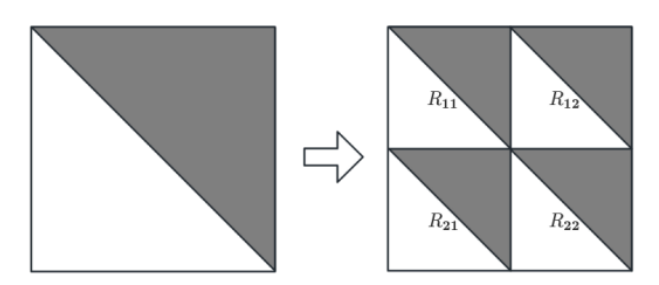
\includegraphics[width=\textwidth]{Upper triangular.png} % Replace with actual file name
%          \caption{Transformation of a $2n \times 2n$ upper triangular matrix.}
%          \label{fig:Upper triangular}
%     \end{minipage}
%     \hfill % Add blank space
%     \begin{minipage}[htbp]{0.45\textwidth}
%         \centering
%         \includegraphics[width=\textwidth]{Upper triangular_decomp.png} % Replace with actual file name
%         \caption{Element permutation form.}
%         \label{fig:Upper triangular_decomp}
%     \end{minipage}
% \end{figure}

% \fi

{\color{red} Is Algorithm 1 is well-known??? or special one for Algorithm 2?}

\begin{algorithm}[H]
        \caption{Matrix Permutation Algorithm} \label{alg:Permutation}
        \textbf{Function:} $B=\text{Permutation}(A,\text{flag})$\\	
        \textbf{Input:}  $ A \in \mathbb{R}^{k \times 2n}$, where flag=0 represents the first submatrix and flag=1 represents the second submatrix.\\
        \textbf{Output:} $B \in \mathbb{R}^{k \times 2n}$ .
    \begin{itemize}
        \item[\textbf{Step 1}]\text{ Recursive stop condition:}\\
            \text{if} $k=2$ \quad return $B=A$;
        \item[\textbf{Step 2}] Initialization:\\
            $k2 = \text{floor}((k+1)/2)$;\\
            $k3 = \text{floor}(k2/2)$;
        \item[\textbf{Step 3}] Add zero rows:\\
            if $\text{mod}(k, 2)=1$ \\
            if flag=1 \quad $A = [\text{zeros}(1, \text{size}(A, 2)); A]$;\\
            else  $A = [A; \text{zeros}(1, \text{size}(A, 2))]$;
        \item[\textbf{Step 4}] Perform swapping:\\
           for $i=1:k3$\\
           if $\text{mod}(k2, 2)=0$ \quad
            $A= \text{swap}(A,2*i,k2+2*(i-1)+1)$;\\
           else
            $A= \text{swap}(A,2*i,k2+2*(i-1)+2)$;
        \item[\textbf{Step 5}] Recursive execution:\\
           $A(1:k2, :) = \text{Permutation}(A(1:k2, :), 0)$;\\
           $A(k2+1:\text{end}, :) = \text{Permutation}(A(k2+1:\text{end}, :), 1)$;
        \item[\textbf{Step 6}] Remove zero rows: \\
           if $\text{mod}(k, 2)=1$ \\
           if flag=1 \quad $B = A(2:\text{end}, :)$;\\
           else $B = A(1:\text{end}-1, :)$;
        \item[\textbf{Step 7}] return $B=A$;
    \end{itemize}
\end{algorithm}

% \begin{theorem}(QR Decomposition)
%     Let $A \in \mathbb{H}_s^{m \times n}$. There exist a unitary matrix $Q \in \mathbb{H}_s^{m \times m}$ and an upper triangular matrix $R \in \mathbb{H}_s^{m \times n}$ such that
%     \begin{equation}
%         A = Q R\label{eq:split QR}
%     \end{equation}
% \end{theorem}

% \iffalse
% \begin{proof}   
% For any matrix $A \in \mathbb{H}_s^{m \times n}$, to prove $A = Q R$, according to the real representation form of the split quaternions, it suffices to prove $A^\sigma = Q^\sigma R^\sigma$, where $Q^\sigma \in \mathbb{R}^{2m\times 2m}$ is unitary and $R^\sigma \in \mathbb{R}^{2m\times 2m}$ is composed of four $m\times n$ upper triangular matrices.

% To ensure that the unitary matrix remains unitary after permutation, we first perform a permutation operation on $A^\sigma$. Let $\hat{A} = P_{m}^T A^\sigma P_{n}$, and then decompose $\hat{A}$ according to the QR decomposition theory of the real matrix, that is,
% \[\hat{A} = \hat{Q} \hat{R}\]
% where $\hat{Q} \in \mathbb{R}^{2m \times 2m}$ is a unitary matrix, and the matrix $\hat{R} \in \mathbb{R}^{2m \times 2n}$ is an upper triangular matrix.

% The upper triangular matrix can be regarded as a special type of $2 \times 2$ block-structured upper triangular matrix. Then, according to Algorithm \ref{alg:Permutation} and Lemma \ref{lemma R4}, $\hat{R}$ can be permuted into a block matrix composed of four upper triangular matrices,
% i.e., \[R^\sigma\triangleq P_{m} \hat{R} P_{n}^T = \begin{bmatrix} R_{11} & R_{12}\\R_{21}& R_{22}\end{bmatrix},\]
% where $R_{ij} (i,j=1,2)$ are upper triangular matrices.

% Thus, we have $\hat{A} = \hat{Q} P_{m}^T R^\sigma P_{n},$
% so $P_{m}^T A^\sigma P_{n} = \hat{Q} P_{m}^T R^\sigma P_{n}$.

% Permute the unitary matrix $\hat{Q}$ in the same way,
% \[Q^\sigma\triangleq P_{m} \hat{Q} P_{m}^T = \begin{bmatrix} Q_{11} & Q_{12}\\Q_{21}& Q_{22}\end{bmatrix},\]
% According to Lemma \ref{unitary matrix}, $Q^\sigma$ is unitary.

% Therefore,
% \begin{equation}
%     A^\sigma = P_{m} \hat{Q} P_{m}^T P_{m} \hat{R} P_{n}^T=\begin{bmatrix} Q_{11} & Q_{12}\\Q_{21}& Q_{22}\end{bmatrix}\begin{bmatrix} R_{11} & R_{12}\\R_{21}& R_{22}\end{bmatrix}=Q^\sigma R^\sigma.
% \end{equation} 
% According to equation \eqref{eq:2.2}, let
% \begin{equation}
%     R = \frac{R_{11} + R_{22}}{2} + \frac{R_{21} - R_{12}}{2}i + \frac{R_{11} - R_{22}}{2}j + \frac{R_{21} + R_{12}}{2}k,
% \end{equation}
% Since $R_{ij}  (i,j=1,2)$ are all upper triangular matrices, $R$ is a split quaternion upper triangular matrix.

% Meanwhile, let
% \begin{equation}
%     Q = \frac{Q_{11} + Q_{22}}{2} + \frac{Q_{21} - Q_{12}}{2}i + \frac{Q_{11} - Q_{22}}{2}j + \frac{Q_{21} + Q_{12}}{2}k,
% \end{equation}
% Thus,
% \begin{equation*}
%      A = Q R.
% \end{equation*}
% \end{proof}
% \fi
\linespread{1.1}
    \begin{algorithm}[htbp]
    \caption{Matrix Permutation Optimization Algorithm}
    \label{alg:Permutation Optimization}
    \textbf{Function:} $B=\text{PermutationOpt}(A,t)$\\
    {\textbf{Input:} \indent  $ A\in \mathbb{R}^{2m\times 2n}$, $t$ is 0 or 1. \\
    {\textbf{Output:}}  $B \in\mathbb{R}^{2m\times 2n}$, $B=PA$ when t is 0, and $B=P^TA$ when t is 1.
          \begin{itemize}
          \raggedright 
          \item[] if $t == 1$\\
          \quad for $i = 1:m$\\
          \qquad $B(2*i-1, :) = A(i, :);$\\
          \qquad $B(2*i, :) = A(m+i, :);$\\
          \quad end\\
          \noindent else\\
          \quad for $i = 1:m$\\
          \qquad $B(i, :) = A(2*i-1, :);$\\
          \qquad $B(m+i, :) = A(2*i, :);$\\
          \quad end\\
          end
          \end{itemize}
    \end{algorithm}

\linespread{1.1}
\begin{algorithm}[htbp] 
        \caption{Compute the QR of Split Quaternion Matrix \(A\)}
        \label{alg:QR}
        \textbf{Function:} $[Q, R]=\text{Split-QR}(A)$\\
        \textbf{Input:} \(A = A_1 + A_2 i + A_3 j + A_4 k \in \mathbb{H}_s^{m\times n}\). \\
        {\textbf{Output:}  }  Unitary matrix \(Q \in \mathbb{H}_s^{m\times m}\), upper triangular matrix \(R \in \mathbb{H}_s^{m\times n}\), satisfying \(Q  R = A\) 
    \begin{itemize}
        \item[\textbf{Step 1}] Real representation of $A$: \(A^\sigma = \begin{bmatrix}
            A_1 + A_3 & -A_2 + A_4 \\ A_2 + A_4 & A_1 - A_3
            \end{bmatrix} \in \mathbb{R}^{2m\times 2n}\);
         \item[\textbf{Step 2}] Compute \(A = P_{m}^T A^\sigma P_{n}\): \\$\hat{A}=\text{PermutationOpt}(A^\sigma,1),$ $\hat{A}=\text{PermutationOpt}(\hat{A}',1),\hat{A}=\hat{A}';$
        \item[\textbf{Step 3}] \([Q,R] = \text{qr}(\hat{A})\);
        \item[\textbf{Step 4}] Compute \(R^\sigma = P_{m}RP_{n}^T\), \(Q^\sigma = P_{m}QP_{m}^T\):\\
        $R=\text{PermutationOpt}(R,0),R=\text{PermutationOpt}(R',0),R^\sigma=R'$\\
        $Q=\text{PermutationOpt}(Q,0),Q=\text{PermutationOpt}(Q',0),Q^\sigma=Q'.$
        \item[\textbf{Step 5}] \(Q_1 = (Q^\sigma(1:m,1:m) + Q^\sigma(m+1:2m,m+1:2m))/2\),
           \(Q_2 = (Q^\sigma(m+1:2m,1:m) - Q^\sigma(1:m,m+1:2m))/2\),
            \(Q_3 = (Q^\sigma(1:m,1:m) - Q^\sigma(m+1:2m,m+1:2m))/2\),
            \(Q_4 = (Q^\sigma(m+1:2m,1:m) + Q^\sigma(1:m,m+1:2m))/2\),
            \(R_1 = (R^\sigma(1:m,1:n) + R^\sigma(m+1:2m,n+1:2n))/2\),
            \(R_2 = (R^\sigma(m+1:2m,1:n) - R^\sigma(1:m,n+1:2n))/2\),
            \(R_3 = (R^\sigma(1:m,1:n) - R^\sigma(m+1:2m,n+1:2n))/2\),
            \(R_4 = (R^\sigma(m+1:2m,1:n) + R^\sigma(1:m,n+1:2n))/2\);
        \item[\textbf{Step 6}] \(Q = Q_1 + Q_2i + Q_3j + Q_4k\),\quad\(R = R_1 + R_2i + R_3j + R_4k\),
        \end{itemize}
\end{algorithm}
% {\color{red}check and polish-The complexity analysis of Algorithm \ref{alg:QR}: For a given split quaternion matrix $A = A_1 + A_2i + A_3j + A_4k \in \mathbb{H}_s^{m\times n}$,  Converting the split quaternion $A$ into the real representation $A^\sigma$ has a computational complexity of $\mathcal{O}(4mn)$ flops. Since the form of matrix $P$ is fixed, when computing $\hat{A}$, $R^\sigma$, and $Q^\sigma$, row and column swapping can be used to reduce computational complexity. Row swapping operations have a computational complexity of $\mathcal{O}(6m)$ flops. The QR decomposition of real matrices has a computational complexity of $\mathcal{O}(mn^2)$ flops. Therefore, the total computational complexity of each iteration of Algorithm \ref{alg:QR} is \(
% \mathcal{O}(mn+6m+mn^2)\).}\\
\textbf{Complexity Analysis:}
% The complexity analysis of Algorithm \ref{alg:QR}: 
{Complexity Analysis:} For a split quaternion matrix \(A = A_1 + A_2i + A_3j + A_4k \in \mathbb{H}_s^{m \times n}\), the computational complexity of Algorithm \ref{alg:QR} is dominated by three components:  

\textbf{1. Real Representation Conversion:}
Constructing the real representation \(A^\sigma \in \mathbb{R}^{2m \times 2n}\) requires  \(4mn\) flops. 

\textbf{2. Permutations On $A, R, Q$:}
Using Algorithm \ref{alg:Permutation Optimization}, which requires approximately \(8m+4n\) flops.


\textbf{3. Real Matrix QR Decomposition:}
The QR decomposition of \(\hat{A} \in \mathbb{R}^{2m \times 2n}\) using Householder reflections dominates the complexity at \(16(mn^2-\frac{n^3}{3})\) flops.

\textbf{Total Complexity}
$$
\underbrace{(4mn)}_{\text{Real Rep.}} + \underbrace{(8m+4n)}_{\substack{\text{Permutation} \\ \text{(optimized)}}} + \underbrace{(16(mn^2-\frac{n^3}{3}))}_{\text{QR}} \approx \boxed{(16(mn^2-\frac{n^3}{3}))}
$$  

\iffalse \textbf{1. Real Representation Conversion:}
Constructing the real representation \(A^\sigma \in \mathbb{R}^{2m \times 2n}\) requires  \(\mathcal{O}(4mn)\) flops. 
\textbf{2. Permutations On $A, R, Q$:}\fi
\iffalse The fixed structure of permutation matrices \(P_m\) and \(P_n\) enables computation of \(\hat{A} = P_m^T A^\sigma P_n\) without explicit matrix multiplication.
By rearranging $A^\sigma$, placing odd rows (columns) first and even rows (columns) last, only $\mathcal{O}(m+n)$ swap operations are needed.

When computing \(\hat{A} = P_m^T A^\sigma P_n\), \(R^\sigma = P_{m}RP_{n}^T\), and \(Q^\sigma = P_{m}QP_{m}^T\), to avoid matrix multiplication, Algorithm 1 is called three times, which requires about \(\mathcal{O}(m+n)\) flops.
\textbf{3. Real Matrix QR Decomposition:}
The QR decomposition of \(\hat{A} \in \mathbb{R}^{2m \times 2n}\) using Householder reflections dominates the complexity at \(\mathcal{O}(mn^2)\) flops.
\fi
% \textbf{Total Complexity:}
% $$
% \underbrace{\mathcal{O}(4mn)}_{\text{Real Rep.}} + \underbrace{\mathcal{O}(4m+2n)}_{\substack{\text{Permutation} \\ \text{(optimized)}}} + \underbrace{\mathcal{O}(mn^2)}_{\text{QR}} \approx \boxed{\mathcal{O}(mn^2)}.
% $$ 

\section{\textbf{Numerical Examples}}
In this section,  we will use the proposed  Algorithm 2 to compute the QR decomposition for split quaternion matrices and apply it to solving a matrix equation.
\begin{example}
    Given a split quaternion matrix $A = A_{0}+A_{1}i+A_{2}j+A_{3}k\in \mathbb{H}_s^{m\times n}$, where
    \begin{equation}
       \begin{cases}
            m = 25,50,\cdots,500;
            n = 25,50,\cdots,500;  \\
            A_{0}=\text{rand}(m,n);
            A_{1}=\text{rand}(m,n); \\
            A_{2}=\text{rand}(m,n);
            A_{3}=\text{rand}(m,n).
        \end{cases} \label{eq:example2}
    \end{equation}
\end{example}
Here, the MATLAB function  $rand(m,n)$ is used to generate an $m \times n$ real matrix with random elements that fall within the interval [0,1]. We executed Algorithm 2 to perform the QR decomposition on $A$, and have computed the CPU time and the relative error
$\epsilon = \frac{\left\|A - Q R\right\|_{F}}{\|A\|_{F}}.$
\iffalse The experimental results are displayed in Figure \ref{fig:cpu times}.\fi
The experimental results from Figure \ref{fig:cpu times} show that Algorithm 2 performs quite well in both speed and accuracy. 
\begin{figure}[htbp]
    \centering
    \begin{minipage}[b]{0.45\textwidth}
        \centering
        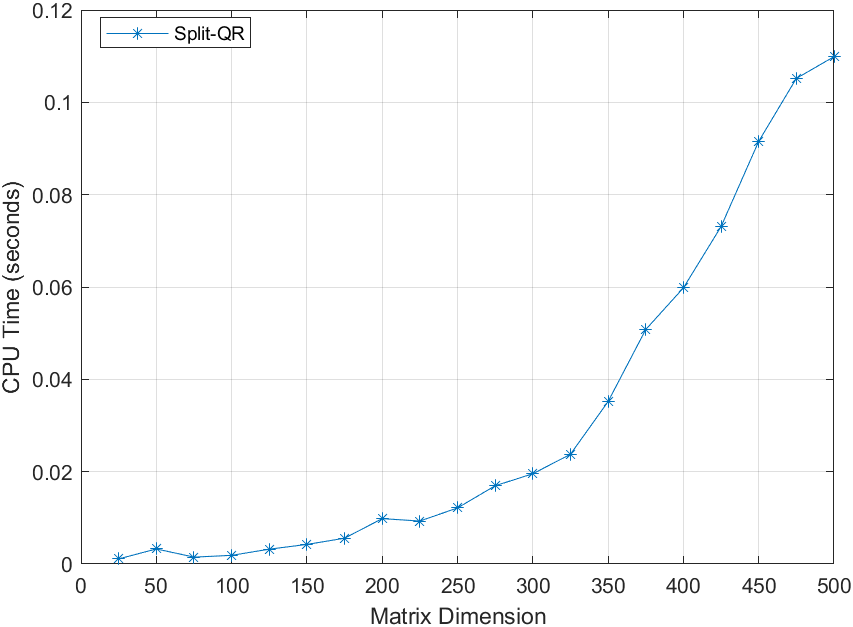
\includegraphics[width=\textwidth]{cpu times.png} % Replace with actual filename
       % \subcaption{(a)}
    \end{minipage}
    \hfill % Add space
    \begin{minipage}[b]{0.45\textwidth}
        \centering
        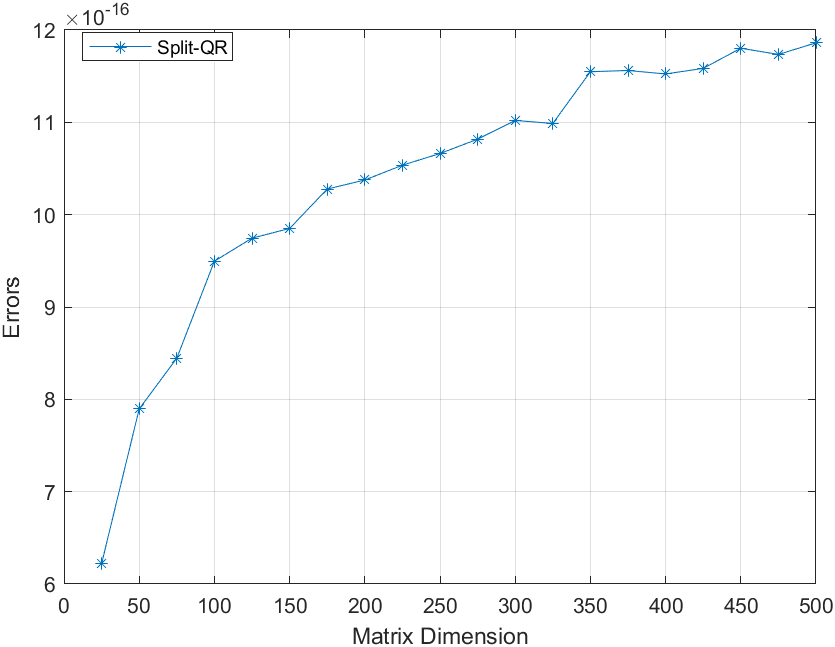
\includegraphics[width=\textwidth]{error.png} % Replace with actual filename
        % \subcaption{(b)}
    \end{minipage}
    % \captionsetup{font=footnotesize}
    \caption{ CPU Time and Error Analysis of the QR Algorithm for Split Quaternion Matrices }
     \label{fig:cpu times}
\end{figure}


Below, we will discuss the application of QR decomposition in solving matrix equation.
\begin{example}
Utilize the QR algorithm to solve the split quaternion matrix equation \(A\dot{X} = \dot{B}\), where
\begin{align*}
A =
\begin{bmatrix}
-4 & -2 & -8 \\
-2 & -2 & -5 \\
7 & -3 & -9
\end{bmatrix} +
\begin{bmatrix}
-1 & -2 & 4 \\
-5 & -8 & -5 \\
-4 & 0 & 6
\end{bmatrix} i +
\begin{bmatrix}
-9 & -6 & -8 \\
-2 & -10 & -5 \\
-10 & -7 & -7
\end{bmatrix} j +
\begin{bmatrix}
-8 & 9 & -3 \\
2 & -6 & 0 \\
8 & 0 & -5
\end{bmatrix} k,
\\
\dot{B} =
\begin{bmatrix}
-9 & -10 & 10 \\
-1 & 10 & 6 \\
-7 & -1 & -10
\end{bmatrix} +
\begin{bmatrix}
4 & 1 & -6 \\
4 & -6 & -3 \\
3 & 6 & 8
\end{bmatrix} i +
\begin{bmatrix}
7 & 2 & 2 \\
-2 & 9 & -4 \\
-4 & 9 & 7
\end{bmatrix} j +
\begin{bmatrix}
-1 & 1 & -3 \\
8 & 5 & -7 \\
-10 & -7 & -4
\end{bmatrix} k.
\\
\end{align*}
\end{example}  
First, perform QR decomposition on $A$ to obtain $Q$ and $R:$
\begin{align*}
Q =
\begin{bmatrix}
-0.514 & -0.047 & -0.344 \\
-0.126 & -0.411 & -0.041 \\
-0.436 & -0.429 & -0.099
\end{bmatrix} +
\begin{bmatrix}
-0.363 & 0.479 & 0.122 \\
0.077 & -0.458 & -0.100 \\
0.383 & -0.194 & 0.138
\end{bmatrix} i \\+
\begin{bmatrix}
-0.236 & -0.062 & -0.155 \\
-0.105 & 0.031 & 0.403 \\
0.262 & 0.178 & -0.296
\end{bmatrix} j +
\begin{bmatrix}
-0.157 & 0.171 & 0.319 \\
-0.250 & -0.133 & 0.577 \\
-0.152 & 0.291 & -0.343
\end{bmatrix} k,\\
R =
\begin{bmatrix}
-3.041 & 3.419 & 10.927 \\
0 & 6.061 & 6.456 \\
0 & 0 & 7.714
\end{bmatrix} +
\begin{bmatrix}
-1.443 & 8.617 & 1.053 \\
0 & 1.847 & -2.947 \\
0 & 0 & -5.025
\end{bmatrix} i \\+
\begin{bmatrix}
20.361 & 5.876 & 6.740 \\
0 & 14.697 & 6.795 \\
0 & 0 & 0.815
\end{bmatrix} j +
\begin{bmatrix}
1.443 & -2.642 & 6.596 \\
0 & -1.847 & -1.528 \\
0 & 0 & 5.025
\end{bmatrix} k.
\end{align*}\\
Thus, the equation can be rewritten as
\begin{equation}
    QRX = B.\label{eq:example1}
\end{equation}
Since \(Q\) is a unitary matrix, \iffalse  \(Q^{-1} = Q^H\),\fi
multiplying both sides of \eqref{eq:example1} by \(Q^H\) from the left yields \(RX = Q^HB\triangleq\hat{B}\),
where
\begin{align*}
\hat{B} =
\begin{bmatrix}
4.981 & 6.383 & 8.076 \\
-2.019 & -1.922 & -1.440 \\
11.356 & 10.929 & -9.652
\end{bmatrix} +
\begin{bmatrix}
-1.144 & -7.725 & 6.206 \\
1.152 & 11.947 & -2.239 \\
-3.761 & 0.482 & -0.749
\end{bmatrix} i \\+
\begin{bmatrix}
-6.136 & -7.249 & -9.693 \\
0.310 & -4.646 & 0.574 \\
1.391 & -2.620 & -3.994
\end{bmatrix} j +
\begin{bmatrix}
11.385 & -4.261 & -2.859 \\
-7.851 & 1.655 & -0.404 \\
-0.653 & 6.826 & 12.841
\end{bmatrix} k.
\end{align*}
Note that \(R\) is an upper triangular matrix, thus   \(RX = Q^HB\triangleq\hat{B}\)  can be solved using back substitution:
 \begin{align*}
\dot{X} =
\begin{bmatrix}
-1.082 & -0.797 & 1.407 \\
-0.316 & -0.028 & 0.749 \\
1.846 & 0.845 & -2.243
\end{bmatrix} +
\begin{bmatrix}
-1.116 & -0.337 & 0.999 \\
-0.423 & -0.961 & 1.907 \\
0.349 & 1.315 & -0.403
\end{bmatrix} i \\+
\begin{bmatrix}
-0.456 & -0.123 & 1.793 \\
-1.222 & -0.449 & 1.810 \\
0.402 & -1.119 & -1.423
\end{bmatrix} j +
\begin{bmatrix}
0.944 & 0.982 & -1.597 \\
0.059 & -0.514 & 0.229 \\
-0.989 & -0.256 & 2.156
\end{bmatrix} k.
\end{align*}
And the relative error is $\frac{\|AX - B\|_F}{\|B\|_F} = 1.2412\times 10^{-15}$.
\iffalse
Potential factors contributing to the effectiveness of this algorithm are as follows: (1) The QR decomposition algorithm omits matrix multiplication operations, instead performing row or column swapping operations, significantly reducing computation time. (2) Although seemingly unstructured, each operational step maintains certain isomorphic relationships, and the computational complexity of the actual operations is typically lower than that of complex operations. Consequently, the computational speed of this method is high.\fi
\iffalse
\section{\textbf{Conclusions}}
By leveraging the special decomposition $A^\sigma = QR_4$ and the unique structure of  real representations for split quaternion matrrces, the QR decomposition of split quaternion matrices was successfully constructed.
-------------------------------------------------------------------
This paper focuses on the problem of QR decomposition for split quaternion matrices, proposing for the first time a research methodology that combines permutation operations with real representation matrices. A QR decomposition theorem suitable for split quaternion matrices is established, and a corresponding QR algorithm is constructed based on it. To validate the effectiveness and superiority of the proposed algorithm, two application examples are provided, with a systematic analysis of the algorithm's computational time consumption and relative error metrics. The experimental results demonstrate that the algorithm exhibits outstanding performance in numerical computations, showing significant advantages in both computational efficiency and accuracy. This provides new theoretical methods and technical approaches for the numerical computation of split quaternion matrices.
\fi

\begin{thebibliography}{99}

\bibitem{Cockle1849} J. Cockle, On systems of algebra involving more than one imaginary; and on equations of the fifth degree, Phil. Mag. 35 (1849) 434–437.
%应用
\bibitem{Hasebe2010} K. Hasebe, Split quaternionic hopf map, quantum hall effect, and twistor theory, Phys. Rev. D 81 (4) (2010) 041702.

\bibitem{Legrand2022} E. Legrand, The geometry of dissipative mechanical systems: Using Jacobi manifolds and the split quaternion algebra, Delft University of
Technology, 2022.

\bibitem{Gogberashvili2022} M. Gogberashvili, (2+1)-Maxwell equations in split quaternions, Physics 4 (1) (2022) 329–363.

\bibitem{Z2022} Z. Özdemir, A kinematic model of the Rytov’s law in the optical fiber via split quaternions: application to electromagnetic theory, Euro. Phys.J. Plus 137 (6) (2022) 1–13.

\bibitem{Wang2023} G. Wang, T. Jiang, V.I. Vasil’ev, Z. Guo, An efficient method for Maxwell’s equations with a discrete double-curl operator in split quaternionic
electromagnetics, Eur. Phys. J. Plus 341 (138) (2023) 1–6.

\bibitem{Yasemin2012} \iffalse Yasemin Alag\"oz, Kh\"ursat Hakan Oral, and Salim Y\"uce.\fi Y. Alag\"oz, K. Oral, and S. Y\"uce. Split quaternion matrices. Miskolc
Mathematical Notes, 13(2):223–232, 2012.

\bibitem{Zhuo2020} X. Liu and Z. He. On the split quaternion matrix equation $AX= B$. Banach Journal
of Mathematical Analysis, 14(1):228–248, 2020.

\bibitem{Xin2019} X. Liu and Y. Zhang. Consistency of Split Quaternion Matrix Equations $AX^* - XB = CY + D$ and $X - AX^*B = CY + D$. Advances in Applied Clifford Algebras, 29:1–20,2019.

\bibitem{Yang2020} X. Liu and Y. Zhang. Least squares \(X = {X^{\eta}}^* \) solutions to split quaternion matrix equation \(AX{A^{\eta}}^*= B\). Mathematical Methods in the Applied Sciences, 43(5):2189–2201, 2020.

\bibitem{Abłamowicz2020} R. Abłamowicz, The Moore–Penrose inverse and singular value decomposition of split quaternions, Adv. Appl. Clifford Algebr. 33 (30) (2020)1–20.

 \bibitem{Zhang2015}Z. Zhang, Z. Jiang, T. Jiang, Algebraic methods for least squares problem in split quaternionic mechanics, Appl. Math. Comput. 269 (2015) 618–625.

\bibitem{Jiang2018}T. Jiang, Z. Zhang, Z. Jiang, Algebraic techniques for eigenvalues and eigenvectors of a split quaternion matrix in split quaternionic mechanics,
Comput. Phys. Comm. 229 (2018) 1–7.

\bibitem{TJiang2018}T. Jiang, Z. Zhang, Z. Jiang, Algebraic techniques for Schrödinger equations in split quaternionic mechanics, Comput. Math. Appl. 75 (2018)2217–2222.

\bibitem{Wang2021}G. Wang, T. Jiang, Z. Guo, D. Zhang, A complex structure-preserving algorithm for split quaternion matrix LDU decomposition in split quaternion
mechanics, Calcolo 58 (34) (2021) 1–15.

\bibitem{Gang2024}G. Wang, T. Jiang, V. Vasil’ev, and Z. Guo. On singular value decomposition
for split quaternion matrices and applications in split quaternionic mechanics. Journal of
Computational and Applied Mathematics, 436:115447, 2024.

\bibitem{TJiang2015} T. Jiang, Z. Jiang, Z. Zhang, Algebraic techniques for diagonalization of a split quaternion matrix in split quaternion mechanics, J. Math. Phys. 56 (2015)083509.

\bibitem{wang}Si, Kai-Wen, Qing-Wen Wang, and Lv-Ming Xie. "A classical system of matrix equations over the split quaternion algebra." Advances in Applied Clifford Algebras 34.5 (2024): 51.

\bibitem{mma}Öztürk, İskender, and Mustafa Özdemir. "On geometric interpretations of split quaternions." Mathematical Methods in the Applied Sciences 46.1 (2023): 408-422.

\bibitem{yuan}Yuan, Shi-Fang, et al. "On Hermitian solutions of the split quaternion matrix equation $AXB+CXD=E$." Advances in Applied Clifford Algebras 27 (2017): 3235-3252.
\end{thebibliography}
\end{document}